% This is samplepaper.tex, a sample chapter demonstrating the
% LLNCS macro package for Springer Computer Science proceedings;
% Version 2.20 of 2017/10/04
%
\documentclass[runningheads]{llncs}
%
\usepackage{graphicx}
\usepackage{paralist}
\usepackage{wrapfig}
% Used for displaying a sample figure. If possible, figure files should
% be included in EPS format.
%
% If you use the hyperref package, please uncomment the following line
% to display URLs in blue roman font according to Springer's eBook style:
% \renewcommand\UrlFont{\color{blue}\rmfamily}

\usepackage[table]{xcolor}% http://ctan.org/pkg/xcolor
\definecolor{lightGreen}{rgb}{0.85, 0.917, 0.827}
\definecolor{grey}{rgb}{128, 128, 128}

\renewcommand{\floatpagefraction}{1}
\renewcommand{\textfraction}{0}

\begin{document}
%
\title{Comparison Matrices of Semantic RESTful APIs Technologies}
%
%\titlerunning{Abbreviated paper title}
% If the paper title is too long for the running head, you can set
% an abbreviated paper title here
%
\author{Antoine Cheron\inst{1}\orcidID{0000-0003-1857-6799} \and
Johann Bourcier\inst{2}\orcidID{1111-2222-3333-4444} \and
Olivier Barais\inst{2}\orcidID{0000-0002-4551-8562} \and
Antoine Michel\inst{1}}
%
\authorrunning{A. Cheron et al.}
% First names are abbreviated in the running head.
% If there are more than two authors, 'et al.' is used.
%
\institute{FABERNOVEL, 46 rue Saint-Lazare F-75010 Paris \email{firstname.lastname@fabernovel.com} \and
Univ Rennes, Inria, CNRS, IRISA 263 Avenue General Leclerc, F-35000 Rennes
\email{firstname.lastname@irisa.fr}}
%\url{https://www.irisa.fr/fr/equipes/diverse}}
%
\maketitle              % typeset the header of the contribution

\begin{abstract}
	
	\vspace*{-0.5cm}
	
Semantic RESTful APIs combine the power of the REST architectural style, the Semantic Web and Linked Data. They picture a world in which Web APIs are easier to browse and more meaningful for humans while also being machine-interpretable, turning them into platforms that developers and companies can build on. We counted 36 technologies that target building such APIs. As there is no one-size-fits-all technology, they have to be combined. This makes selecting the appropriate set of technologies to a specific context a difficult task for architects and developers. So, how the selection of such a set of technologies can be eased?
In this paper we propose a comparison matrix of Semantic RESTful APIs enabling technologies. It is based on the analysis of the differences and commonalities between existing technologies. It intends to help developers and architects in making an informed decision on the technologies to use. It also highlights the limitations of state-of-the-art technologies from which open challenges are derived.

\vspace*{-0.2cm}
\keywords{Semantic Web\and REST\and Web API\and comparison\and Linked Data}
\end{abstract}
%
\section{Introduction}

Today, RESTful APIs \cite{FieldingThesis} have become the de-facto standard for building web applications. The main reason behind this popularity lies in the appropriate trade-off between the facility to build such applications and the benefits provided by this approach in such an opened large-scale distributed system: evolutivity, scalability and loose-coupling. However, 95\% of Web APIs are not RESTful ~\cite{10.1007/978-3-319-38791-8_2} as they claim.

Until today, no single standard has emerged to design truly RESTful APIs. Consequently, software architects are facing the challenge of selecting the right technologies for the design and implementation of these systems. Typically, a software architect has to select the right interface description language, interchange format and framework to ease the development of such APIs.

In addition, a new trend has recently emerged to create RESTful APIs that carry their own semantics, they are called Semantic RESTful APIs~\cite{7195633}. It is a vision that proposes to make fully REST-compliant APIs compatible with the Semantic Web ~\cite{TheSemanticWeb} and Linked Data~\cite{LinkedDataPrinciples}. From our experience at FABERNOVEL, we found that building such APIs does not require much more effort than truly RESTful systems, whereas it offers great benefits, such as loose-coupling, automated API mash-ups~\cite{benslimane2008services}, machine-interpretability and very powerful querying. 

% TODO: add a word on the questionnaire sent to developers to gather their REX on choosing hypermedia and Linked Data technologies
However, the design of semantic RESTful APIs considerably increases the complexity for the architect to choose the appropriate technology. Indeed, the specific criteria and properties to be taken into account when choosing an IDL, an exchange format and a framework are not explicit. A decision matrix is missing that would allow the architect to understand the consequences of a design decision, i.e. the characteristics and limitations of each approach.
 
In this paper, we propose to fill this gap by providing decision matrices that help architects to choose the technologies that will best meet their needs. The main contributions of this paper are:

\begin{itemize}
    \item three comparison matrices of interchange formats, interface description languages and frameworks that help choosing appropriate technologies to build Semantic RESTful APIs
    \item key features that are missing from state-of-the-art technologies to assist and make more beneficial the creation of Semantic RESTful APIs
\end{itemize}

Based on these comparison matrices, we draw the outline of a research road-map to ease the adoption of Semantic RESTful APIs in industry.

The remainder of this paper is organized as follows. Section \ref{sec:background} provides the required background on semantic REST API and the reference maturity level to choose the functionality level of an API along with its limitation. The two following sections describe our comparison matrices and an illustration example that highlights the benefits of our proposition. Finally section \ref{sec:discussion} discusses the role of the existing frameworks to build REST APIs. 

\section{Background} \label{sec:background}

% JOHANN -> TODO. I merged section 2 and 3 in this file.

% TODO - From reviewer 2 : Most of the background should be already known by readers and can be shortened/omitted. RESTful technologies are of daily use for anyone interested on Web Technologies.

% TODO - From reviewer 2 : Do not spend an entire section on someone's else work. You can introduce the maturity model as part of the background (even omitting the figure), provide appropriate references and discuss its disadvantages.
% Antoine -> I think we should keep the figure of the maturity model, it is a very good visual helper to its understanding.

This section describes the main concepts related to the design and implementation of Semantic Restful Web APIs and the process of selecting an API functionality.

% Antoine: to me, we can remove this subsection
%\subsection{REST}

%The REST architectural style imposes constraints on the design of a distributed system to guarantee the following properties: extensibility, evolution, loose-coupling and easy browsing~\cite{FieldingThesis}. To achieve this goal, it proposes six constraints: (i) \textit{client-server}, (ii) \textit{stateless}, (iii) \textit{cache}, (iv) \textit{uniform interface}, (v) \textit{layered system} and (vi) \textit{code-on-demand}. The latter is optional. The \textit{uniform interface} constraint is itself defined by four constraints: (i) \textit{unique identification of resources}, (ii) \textit{manipulation of resources through representations}, (iii) \textit{self-descriptive messages} and (iv) \textit{hypermedia as the engine of application state (HATEOAS)}.

% Antoine: to me, we can remove this subsection
%\subsection{Semantic Web and Linked Data}

%The Semantic Web~\cite{TheSemanticWeb} envisions the Web as an open platform, where information is machine processable and unstructured. This vision allows to create complex queries gathering information on the whole Web, which would otherwise be impossible.  It also allows global knowledge to grow quickly and easily because this global knowledge can be distributed among the different stakeholders. To achieve this goal, the Semantic Web community offers a unique and comprehensive set of technologies, including a data model, query language, framework, database, ontological languages, exchange formats and more.

%The principles of Linked Data are an extension of the Semantic Web. They advise using meaningful URIs to name things and including links to other resources to create an interconnected information structure. 

%With Linked Data, the Semantic Web is becoming closer to the uniform interface of REST systems since these principles are equivalent: namely (i) \textit{unique identification of resources}, (ii) \textit{manipulation of resources through representations} and (iii) \textit{hypermedia as the engine of application state (HATEOAS)}. 

% Antoine: to me, this section should stay. The subject is not well known. Scholar gives 91 results for "semantic rest" and 171 for "semantic restful".
\paragraph{Semantic RESTful services}
Combining REST with Semantic Web and Linked Data is a promising path since it enables the description of APIs that can change without breaking client applications. These APIs advertise their available state transitions, therefore enabling automatic composition to create high level services \cite{alarcon2015rest}. Smart software agents can then automatically discover the suite of operations to realize complex workflows and even make APIs compatible with voice assistants. This is achieved by semantically enriching the data and operations of REST systems with Semantic Web ontology technologies and by linking resources to other resources.

% Antoine: to me, this section should stay in a shortened version because precision on the implementation, the types and guards are not used in the rest of the paper.
%\subsection{Resource Model}

%A resource model aims to model REST systems in which resources are the central element. A resource is any kind of named element, e.g. a photo, a spreadsheet or a table. It has representations, e.g. in the form of a JSON document or even a jpg image, and state transitions, which availability depends on the current state of the system. State transitions can be viewed as operations, either on the resource itself or on others. A common transition refers to a reading operation of another resource. This transition creates a link between the two resources. In the rest of this paper, operations on the resource itself are called operations while operations on other resources are called links.

%It is important to note that, the notion of resources cannot be mapped to the notion of class or entity in an object model. Indeed, the distinction between the notion of class and role does not necessarily exist in a resource-oriented approach. As an illustration, \emph{Users} is a different type of resource than \emph{User}.

%as opposed to classes in object-oriented modeling, a collection of resources of type T is another kind of resource than T. As an illustration, \emph{Users} is a different type of resource than \emph{User}.

%A resource type behavior may be described with a state machine, as presented in \cite{Schreier:2011:MRA:1967428.1967434}. If a resource's state change, the resource stays of the same type, even if the implementation represents different states with different classes. Each state may have some operations only available in the given state, and others available in every states. Operations have guards, computed from the values of the resource properties and the context, for example the currently connected user.

%Everything can be modeled as resources, including descriptions of operations that could then be used to generate actual HTTP operations at runtime. This way, the number of concepts is lowered and the model contain its own description, which leads to systems where the data and their descriptions can be accessed through a single mechanism.

\subsection{Selecting an API functionality level}\label{sec:maturityLevel}

The first step an architect faces when designing a Web API is to select the features to support.
Architects use a maturity model to help them decide on the supported features. In general, a maturity model is a scale that represents to what level a technology complies with a given architecture. To reach a level, a technology must meet each constraint of the previous levels and of the targeted level.
Currently, the most used maturity model in industry is the Richardson Maturity Model \cite{RichardsonMaturityModel}, which targets building REST APIs. However, we recommend using the WS3 maturity model \cite{7195633} as it extends the Richardson one, and SoHA \cite{SoHA}, with Semantic REST API-enabling constraints.

\paragraph{The WS3 maturity model}

In \cite{7195633}, authors describe the WS3 maturity model for classifying Semantic REST Web APIs. WS3 aims at promoting the adherence to REST architectural principles and the adoption of Semantic Web technology to improve the design, reuse, integration and documentation of Web APIs. It classifies APIs along three independent dimensions: \textit{design}, \textit{profile} and \textit{semantic}, as shown in Fig. \ref{WS3}.

\begin{figure}[ht]
  \caption{WS3 Maturity Model (from \cite{7195633})}
  \centering
  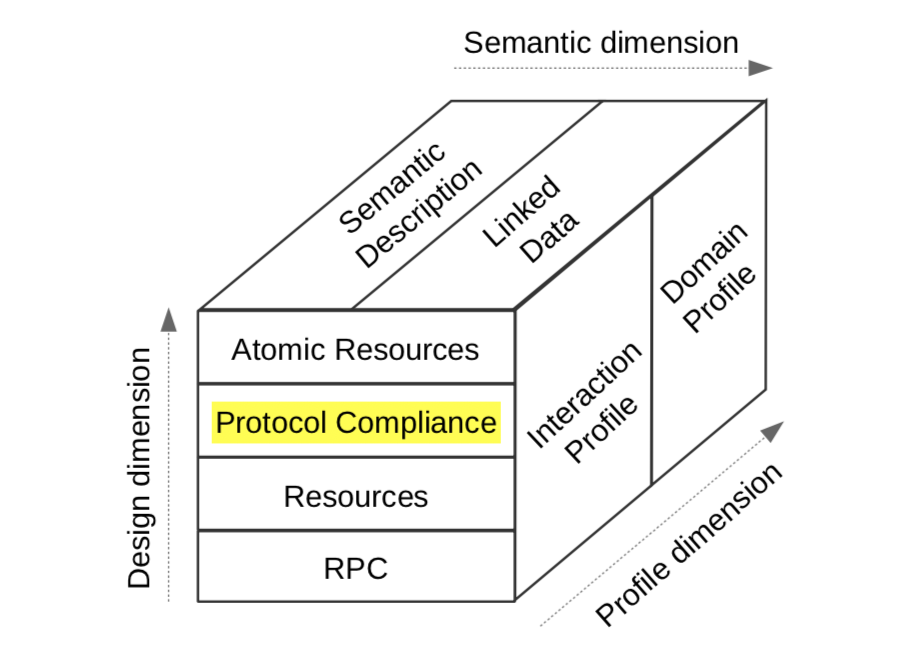
\includegraphics[width=0.47\textwidth]{figures/ws3-maturity-model.png}
  \label{WS3}
\end{figure}

The design dimension represents the different modeling strategies adopted for designing the technical access to a Web API through four levels. The first three levels are similar to the first three levels of the Richardson maturity model. The four levels are (i) RPC-like, (ii) resources have dedicated URI and the API is stateless, (iii) operations on a resource are mapped to HTTP verbs in compliance with the protocol and (iv) the smallest data unit that can be handled by operations is the resource.

The Profile dimension reflects the quality of documentation provided by the Web API through two levels. It takes into account only documentations that can be interpreted by software agents. The first level, interaction profile, requires the description of all available HTTP operations and how to trigger them. The second and final level, the domain profile, requires the description of domain specific details such as the order of operation execution, pre- and post-conditions, business constraints, etc. This level may be reached by providing hypermedia controls at runtime.
% From Antoine: sentence "It takes into account only documentations that can be interpreted by software agents" important to keep

The Semantic dimension represents the use of semantic technologies through two levels. To reach the Semantic Description level, an API must semantically describe properties and operations of resources. Next level, Linked Data, is reach when the API semantically describes relationships between resources.

\paragraph{Usage}

In their paper, Salvadori \emph{et al.} propose to rate systems along each dimension independently, with a score going from 0 to the number of levels in the dimension.

For example, a non-documented API with no semantic support that reach level 3 of the Richardson Maturity Model will be rated D3-S0-P0. This means that the API reach the Protocol Compliance level of the Domain dimension and no level of both the Semantic and Profile dimensions.

%For another example, we consider building an API that supports HATEOAS and that provides a swagger-like documentation in the messages at runtime. HATEOAS is used to document available state transitions and to advertise users of the next operations to trigger in order to complete a given business process. This API is rated D3-S0-P2.

A system that supports HATEOAS and provides a swagger-like documentation along with the data, to inform the user of available state transitions, and of the operations to trigger to complete a given business process, is rated D3-S0-P2.

\paragraph{Discussion}

The WS3 maturity model is today the most complete maturity model to classify web semantic Rest API. Nevertheless, from our experience at FABERNOVEL, we noticed two limitations to the applicability of the maturity model to a wider audience. These limitations are related to the Atomic Resources level and the abstraction chosen by the authors.

The Atomic resources constraint requires that the smallest data unit that can be handled by operations is the resource. Let us consider an API handling insurance contracts, that is readable and allows updating the postal address, email address and insurance manager, respecting the Atomic Resources constraint.  Two solutions can be considered. The first one is to create one resource, where every properties can be modified at once, which creates the risk that if two users want to modify two different information at the same time, only one may be made. With this solution, the API would have two operations. The second solution is to create four resources: one for the contract, one for the email address, one for the postal address and one for the manager. The API would have seven operations. The best trade-off would be to create one resource with four operations: (i) read, (ii) update email, (iii) update postal address and (iv) update manager. This solution lowers concurrency risks, the complexity for users and developers is in the middle of the two solutions offered by the Atomic Resources constraint and operations have a more meaningful name.

The second limitation relates to the granularity of the maturity levels. Indeed, each level implies more than one feature. This granularity allows for a coarse-grained categorization of systems. However, to precisely differentiate systems based on the features they implement, a deeper study is needed. Given two systems that reach P1, which means they describe all available HTTP operations and how to trigger them, one might also describe its authentication process and errors whereas the second does not. And yet they reach the same maturity level. As a second example, we consider two systems that describe HTTP operations and domain details such as the order of operations and the authentication process. One might support hypermedia controls whereas the other one has an OpenAPI documentation. These two features allow to reach the same maturity level: P2, even though they make a big difference from the client point of view.

\vspace*{-0.5cm}
\section{Comparison Matrices}\label{sec:matrix}

\vspace*{-0.3cm}
We propose three detailed matrices which address the limits of WS3 identified in the previous section. 
The proposed matrices enable the comparison of technologies along a set of precise criteria to highlight their differences. 
These matrices extend the WS3 level by adding some new criteria which are used in practice(see section \ref{sec:insight}) and not linked to any WS3 level.

\vspace*{-0.2cm}
\subsection{Insights from developers and architects}\label{sec:insight}

We interviewed 14 developers and architects from FABERNOVEL and clients on their experience with Semantic REST technologies. Raw results and the analysis are available online\footnote{\url{https://github.com/AntoineCheron/comparison-matrices-semantic-rest-api-techno}}. Our key findings are:
\begin{itemize}
 \item \textit{Selecting the technology:} 10 respondents have already built Semantic REST APIs: \textbf{30\%} spent more than two weeks selecting the technologies; \textbf{80\%} reported that the most difficult task was to understand the feature provided by each technology.
 \item \textit{Interchange Formats:} \textbf{6 out of 7} did not find a technology providing all required features (most often the missing features were the description of HTTP operations with their data model (3/8) and the Linked Data (2/8)). 
 \item \textit{Interface description languages:} All respondents said that none of them provide all required features (60\% said they lack the ability to describe links to other resources and business constraints; and 20\% of them would like to model the resources as finite state machines (FSM)).
 \item \textit{Frameworks:} 6 out of 7 reported that no framework offered the required feature. The missing features are related to the auto-documentation of the API, the automatic generation of link and a mechanism to model resources as FSM.
 \item \textit{Technology score:} The median value of the score is 2/5.
 %\item \textit{??:} have never built such APIs, none know the Semantic Web or Linked Data. One sees not interest in building HATEOAS APIs, another considers that the technologies are too difficult to find and the last one says that it is too time consuming.
\end{itemize}

These results emphasize the difficulties for selecting technology associated to Semantic REST APIs. They also highlight that these technologies are not yet mature and give a rough idea of the missing features.

\subsection{Comparison Matrices Design Methodology}

The design of our comparison matrices follows a 5 steps sequential process: \textit{(i)} \textbf{search} for candidate technologies, \textit{(ii)} \textbf{select} candidate technologies, \textit{(iii)} \textbf{read} carefully each candidate technology, \textit{(iv)} \textbf{elaborate fine grain criteria} to characterize and differentiate technologies, \textit{(v)} \textbf{verification} that the elaborated criteria highlighted the differences between technologies. We looped on step \textit{(iv)} and \textit{(v)} to avoid duplicating criteria or hiding important details.

The research of candidate technologies (step i) was done by:

\begin{enumerate}
    \item Searching Google and Google Scholar for Semantic REST Technologies using compositions of keywords from the set: ["web", "semantic", "restful", "rest", "service", "API", "interface", "description", "documentation", "language", "modeling", "hypermedia", "document", "format", "RDF", "data-interchange", "linked data", "hateoas", "rest api", "framework"];
    \item Searching Google Scholar for tools automating tasks from services description, using keywords: "matchmakers", "service composition", "service discovery", "rest service analysis", "automated mashups", we then selected papers and technologies from their references and the papers that cite those we selected;
    \item Searching the proceedings of ICWE and WS-REST. 
\end{enumerate}

We selected 81 papers, standards, articles and web pages (step ii) from their abstract or introduction. We selected documents that were specifications of interface description languages or models, frameworks supporting HATEOAS features, interchange formats that support RDF or HATEOAS features, comparisons between these technologies or tools leveraging them. Frameworks to build Semantic Web Services were excluded because they are based on triples, which are too far from the resource-oriented design of REST. We opened our research to technologies from the 1990s to today and retained those that are still available today.

As a next step, we read the specification of each chosen technology (step iii) and elaborate classification criteria (step iv). We included those of the H~Factor~\footnote{\url{http://amundsen.com/hypermedia/hfactor/}} which \textit{is a measurement of the level of hypermedia support and sophistication of a media-type}. Others were carefully designed to highlight differences between technologies, based on the core design of the technologies, the features they provide and the details of the WS3 maturity model. All material is available online\footnote{\url{https://github.com/AntoineCheron/comparison-matrices-semantic-rest-api-techno}}.

As a final step (step v), we read the specifications again to verify results and validate that the selected criteria highlighted differences and commonalities well.

\paragraph{Popularity criteria}

We defined a popularity criteria to provide a rough idea of the community support and the likelihood of the technology to last in time. It respects the following rules: 
\begin{inparadesc}
    \item [0 -] Not enough to reach 1;
    \item [1 -] More than 100 questions on stack overflow AND (2500+ NPM weekly downloads OR 100+ maven usages);
    \item [2 -] More than 400 questions on stack overflow AND (more than 500.000 total downloads OR more than 15.000 NPM weekly downloads OR more than 500 maven usages).
\end{inparadesc}

\subsection{Interface Description Languages}

Interface Description Languages (IDLs) provide a vocabulary to document domain, functional and non-functional aspects of an API.
We identified 16 candidates that are classified according to 31 criteria in Fig~\ref{idl-matrix}. Among them, 4 are meta-models from conference papers \cite{10.1109/ICWS.2014.30} \cite{Rapido} \cite{Schreier:2011:MRA:1967428.1967434} \cite{10.1007/978-3-642-22233-7_24}. The 11 others are open-source projects or W3C recommendations.

In \cite{Rapido} authors present a tool to sketch CRUD or Hypermedia APIs. On the latter mode, users sketch the application using state-machines and then obtain a description in the HAL or Collection+JSON format.
\cite{Schreier:2011:MRA:1967428.1967434} models each resource type as a finite-state-machine with deterministic transitions, and conditions to inform about the availability of transition. However, they are not modeled in more details, which do not make them machine-interpretable.
In~\cite{10.1007/978-3-642-22233-7_24}, authors propose to model systems as non-deterministic state machines. This method thus makes software agents unable to discover the set of messages to exchange in order to make an operation available.
Haupt et al.~\cite{10.1109/ICWS.2014.30} propose a multi-layered model that separates the domain model from the URI model. However, resources have a fixed model, which does not allow them to have a data model adapted to each state.

It is important to note than when \textbf{IDLs and interchange formats} are both \textbf{compatible with RDF}, they can be combined to form a file format usable as data-interchange format and IDL. This has great benefits to lower the overall complexity and increase the evolvability of the system.

% FIGURE OF THE IDL CLASSIFICATION
\begin{figure*}[!ht]
\caption{Interface Description Languages Comparison Matrix}
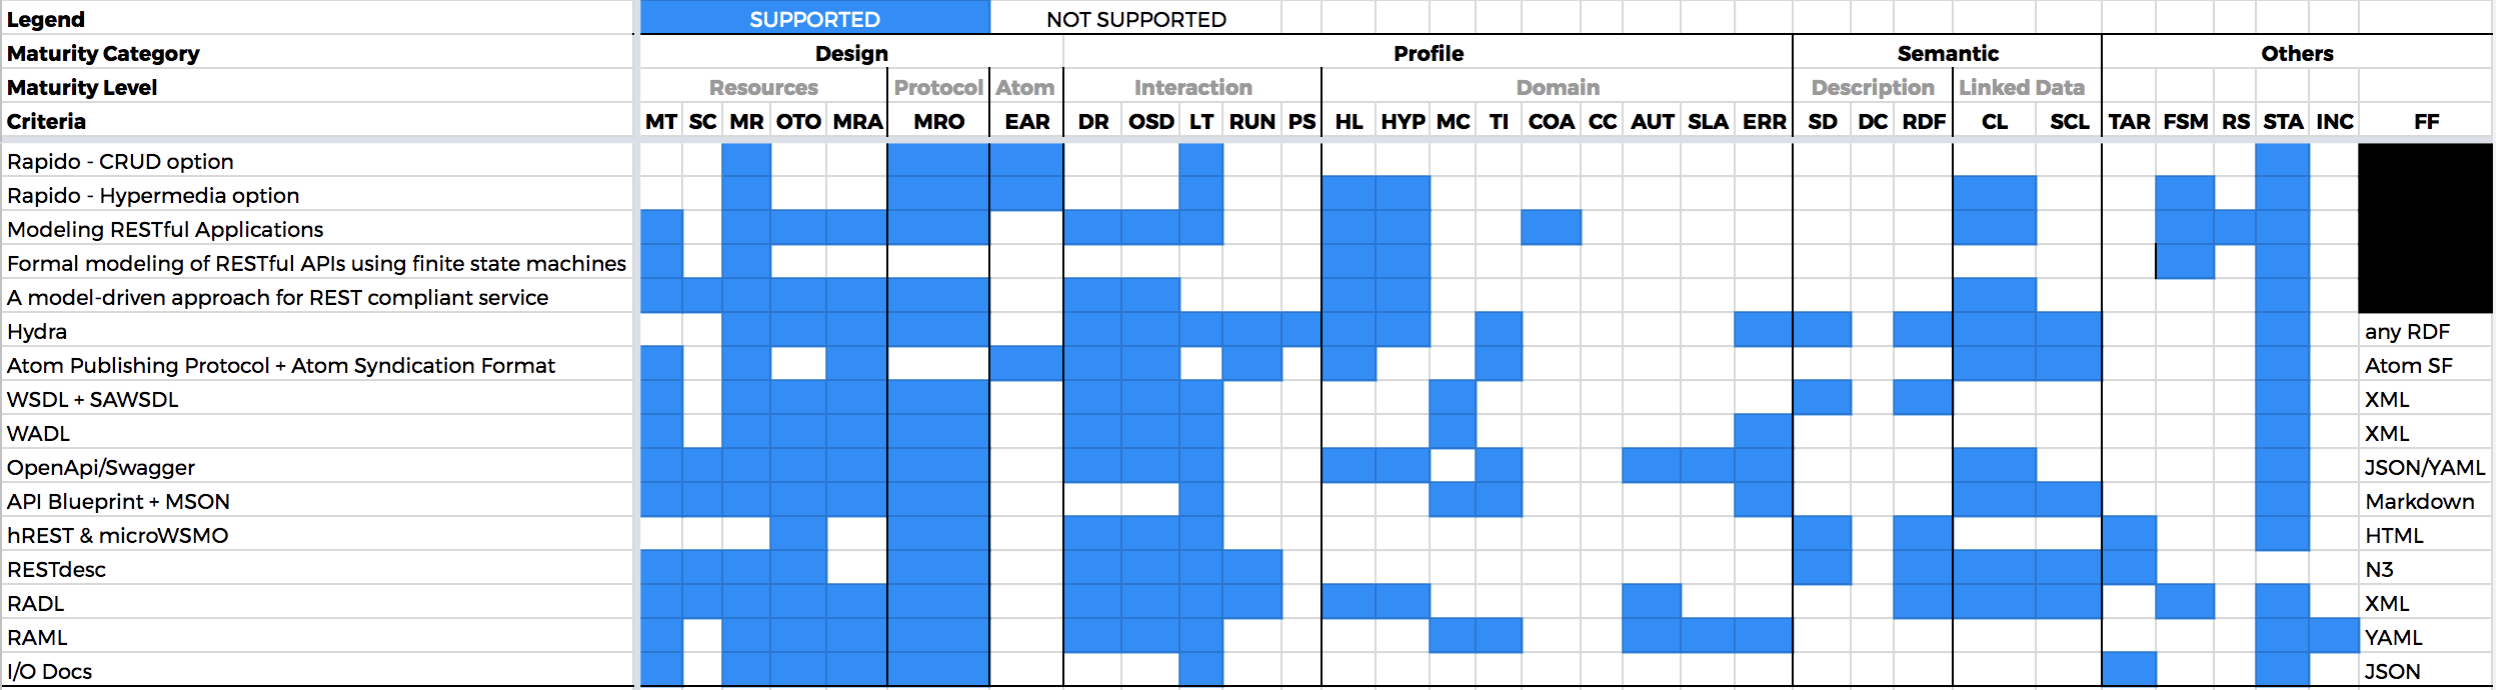
\includegraphics[width=1\textwidth]{figures/IDL.png}
\label{idl-matrix}
\vspace{-1.2cm}
\end{figure*}

\subsubsection*{Synthesis}

First, the matrix highlights the fact that most technologies help building mature systems on the \textit{design} dimension and \textit{interaction profile} level of the \textit{profile} dimension, D3-P1 following the WS3 categories.
On the other hand on the \textit{semantic} dimension, we notice that 5/16 technologies support the use of RDF vocabulary, which allows to build Linked Data APIs. As a reminder, this is required to reach full Semantic REST compliance.
Moreover, by supporting the use of RDF vocabulary, IDLs can be enriched to reach a higher level of maturity.

Among the technologies, four can be distinguished by the number of criteria they meet: Hydra (18), RADL (18), OpenAPI (17) and RESTdesc (17).
OpenAPI is the only one that has no support for RDF. Thus, it helps in building systems up to D3-P2-S0 on the WS3 scale.
On the other hand, Hydra, RADL and RESTdesc support the use of RDF vocabulary, which makes these technologies better suited to build systems that are mature on the semantic dimension.

\textit{Towards HATEOAS APIs}
From the matrix, we notice that most technologies target the documentation of the API in a single, non-splittable file. Hence, they are not suited to provide hypermedia controls at runtime.

On the other hand, only one approach, \cite{Schreier:2011:MRA:1967428.1967434}, supports the description of the conditions that determine the availability of a link, and none makes this meta-data machine-interpretable. This makes software agents unable to find a way to make an operation available when it is not.

\textit{Towards better-documented APIs}
Only four technologies support the description of business constraints although it lowers coupling and improves user experience, e.g., with the automatic generation of forms with client-side validation.

Finally, we note that most scientific publications recommend the modeling of RESTful systems as state-machines whereas open-sourced or W3C IDL authors don't consider this design method. And yet, the use of deterministic state-machines eases determining the availability of operations on a resource.

\subsection{Data-interchange formats}

Data-interchange formats provide a data-structure, a vocabulary and a layout to represent a resource and its meta-data at runtime. When the API do not need to send meta-data, JSON and XML are the two formats widely used in the industry.

On the other side, when the system to build have to support a hypermedia interchange format, none is considered as a standard today. We selected 11 candidate technologies, which are classified in Fig.~\ref{interchange-formats-matrix} according to 24 criteria. JSON is included for comparison purpose.

% FIGURE OF THE INTERCHANGE FORMATS CLASSIFICATION
\begin{figure*}[!ht]
\caption{Data-interchange Formats Comparison Matrix}
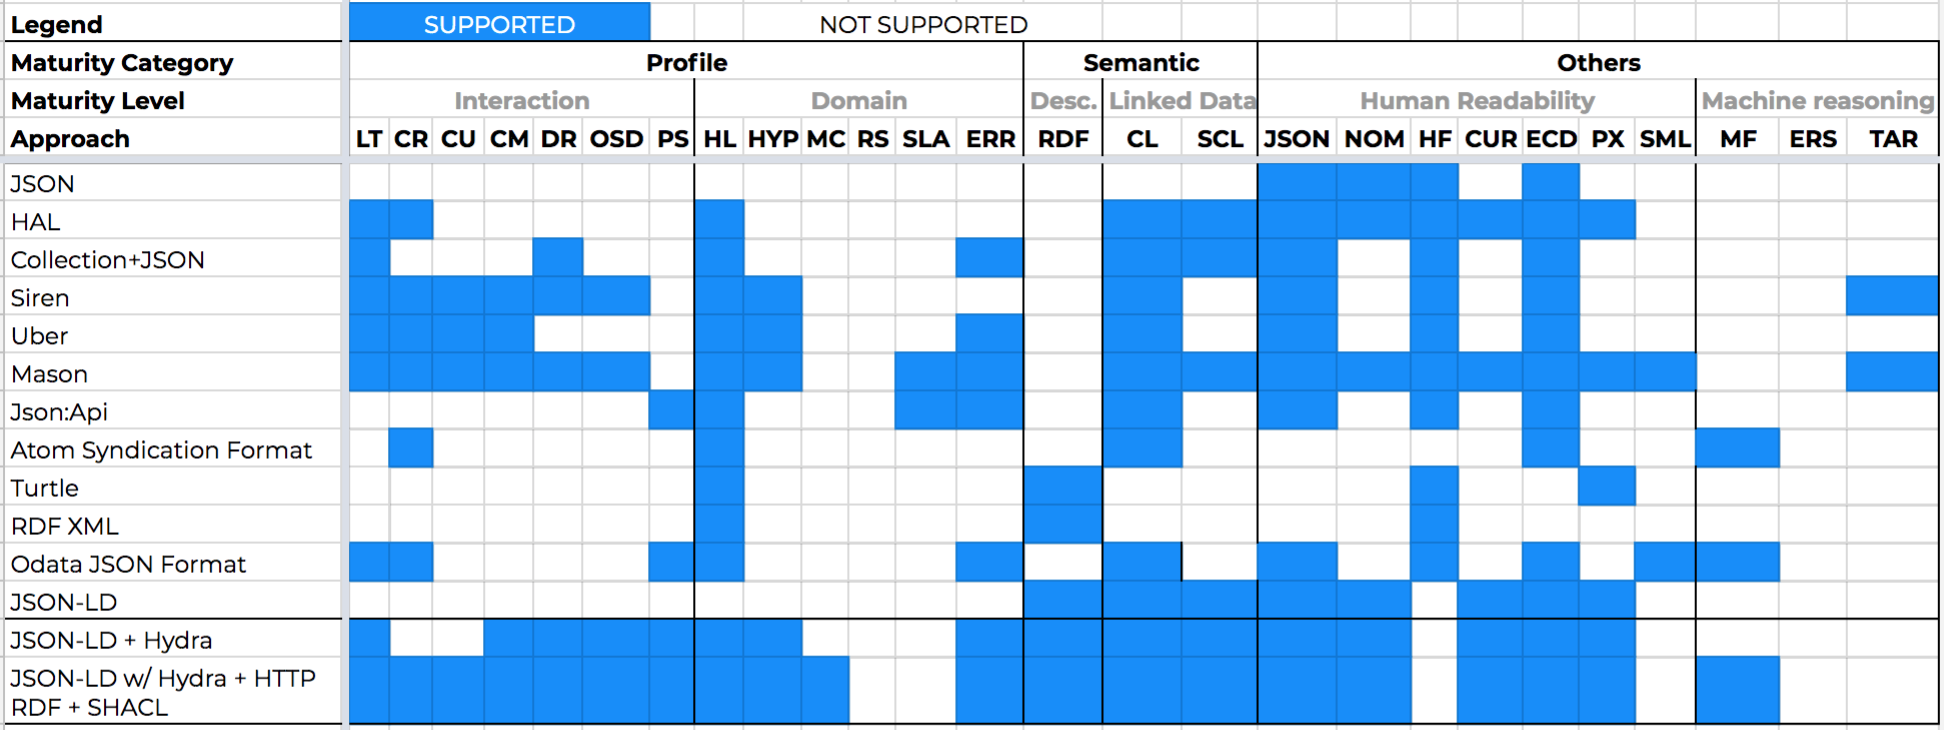
\includegraphics[width=1\textwidth]{figures/DIF.png}
\label{interchange-formats-matrix}
\vspace*{-0.7cm}
\end{figure*}

\subsubsection*{Synthesis}
First, from this matrix, we notice that formats can be differentiated based on their compatibility with RDF. Indeed, RDF formats (Turtle, RDF XML and JSON-LD) can be enriched with RDF vocabularies. This is why they propose very few features by default. To depict what is possible to achieve by combining vocabularies with a RDF format, we selected two vocabularies: Hydra and SHACL, an RDF schema validation vocabulary, that we combined with JSON-LD and evaluated it. As a result, it matches 12 more criteria than JSON-LD alone.
From this, we infer that combining RDF formats with vocabularies allow building mature Semantic REST systems. However, this requires additional effort to find relevant vocabularies.
On the other hand, non-RDF formats help building systems that can be mature on the \textit{profile} dimension but not on the \textit{semantic} dimension.

Furthermore, the matrix shows that no format supports the description of constraints despite the fact that it can be leveraged to reduce coupling and improve the user-experience.

Finally, it highlights that no format advertise the state of the resource even though most scientific approaches we found describe REST APIs as state-machines.

\subsection{Implementation Frameworks}

Implementation frameworks are software libraries that guide developers through the implementation of Web APIs. We limit the comparison to frameworks that claim to support HATEOAS. We identified six frameworks that do so. Frameworks to build Semantic Web Services are excluded because their triple-centric approach is too far from REST.

Among selected papers, in \cite{salvadori2014framework} authors propose \textit{Hypermedia Web API Support}, a Java framework based on JAX-RS 2.0 that offers annotations to semantically describe REST APIs. The end result is the description of the whole API in a JSON-LD document enriched with the Hydra vocabulary. Unfortunately, the framework is not available in Maven Central. In \cite{parastatidis2010role} Parastatidis et al. present \textit{Restfulie}, a framework that uses resources, state transitions and content-negotiation as its core building blocks. We found 4 other frameworks that support HATEOAS features. They are all classified in Fig.~\ref{frameworks-matrix} according to 23 criteria.

% FIGURE OF THE IMPLEMENTATION FRAMEWORKS CLASSIFICATION
\begin{figure*}[!ht]
\caption{Implementation Frameworks Comparison Matrix}
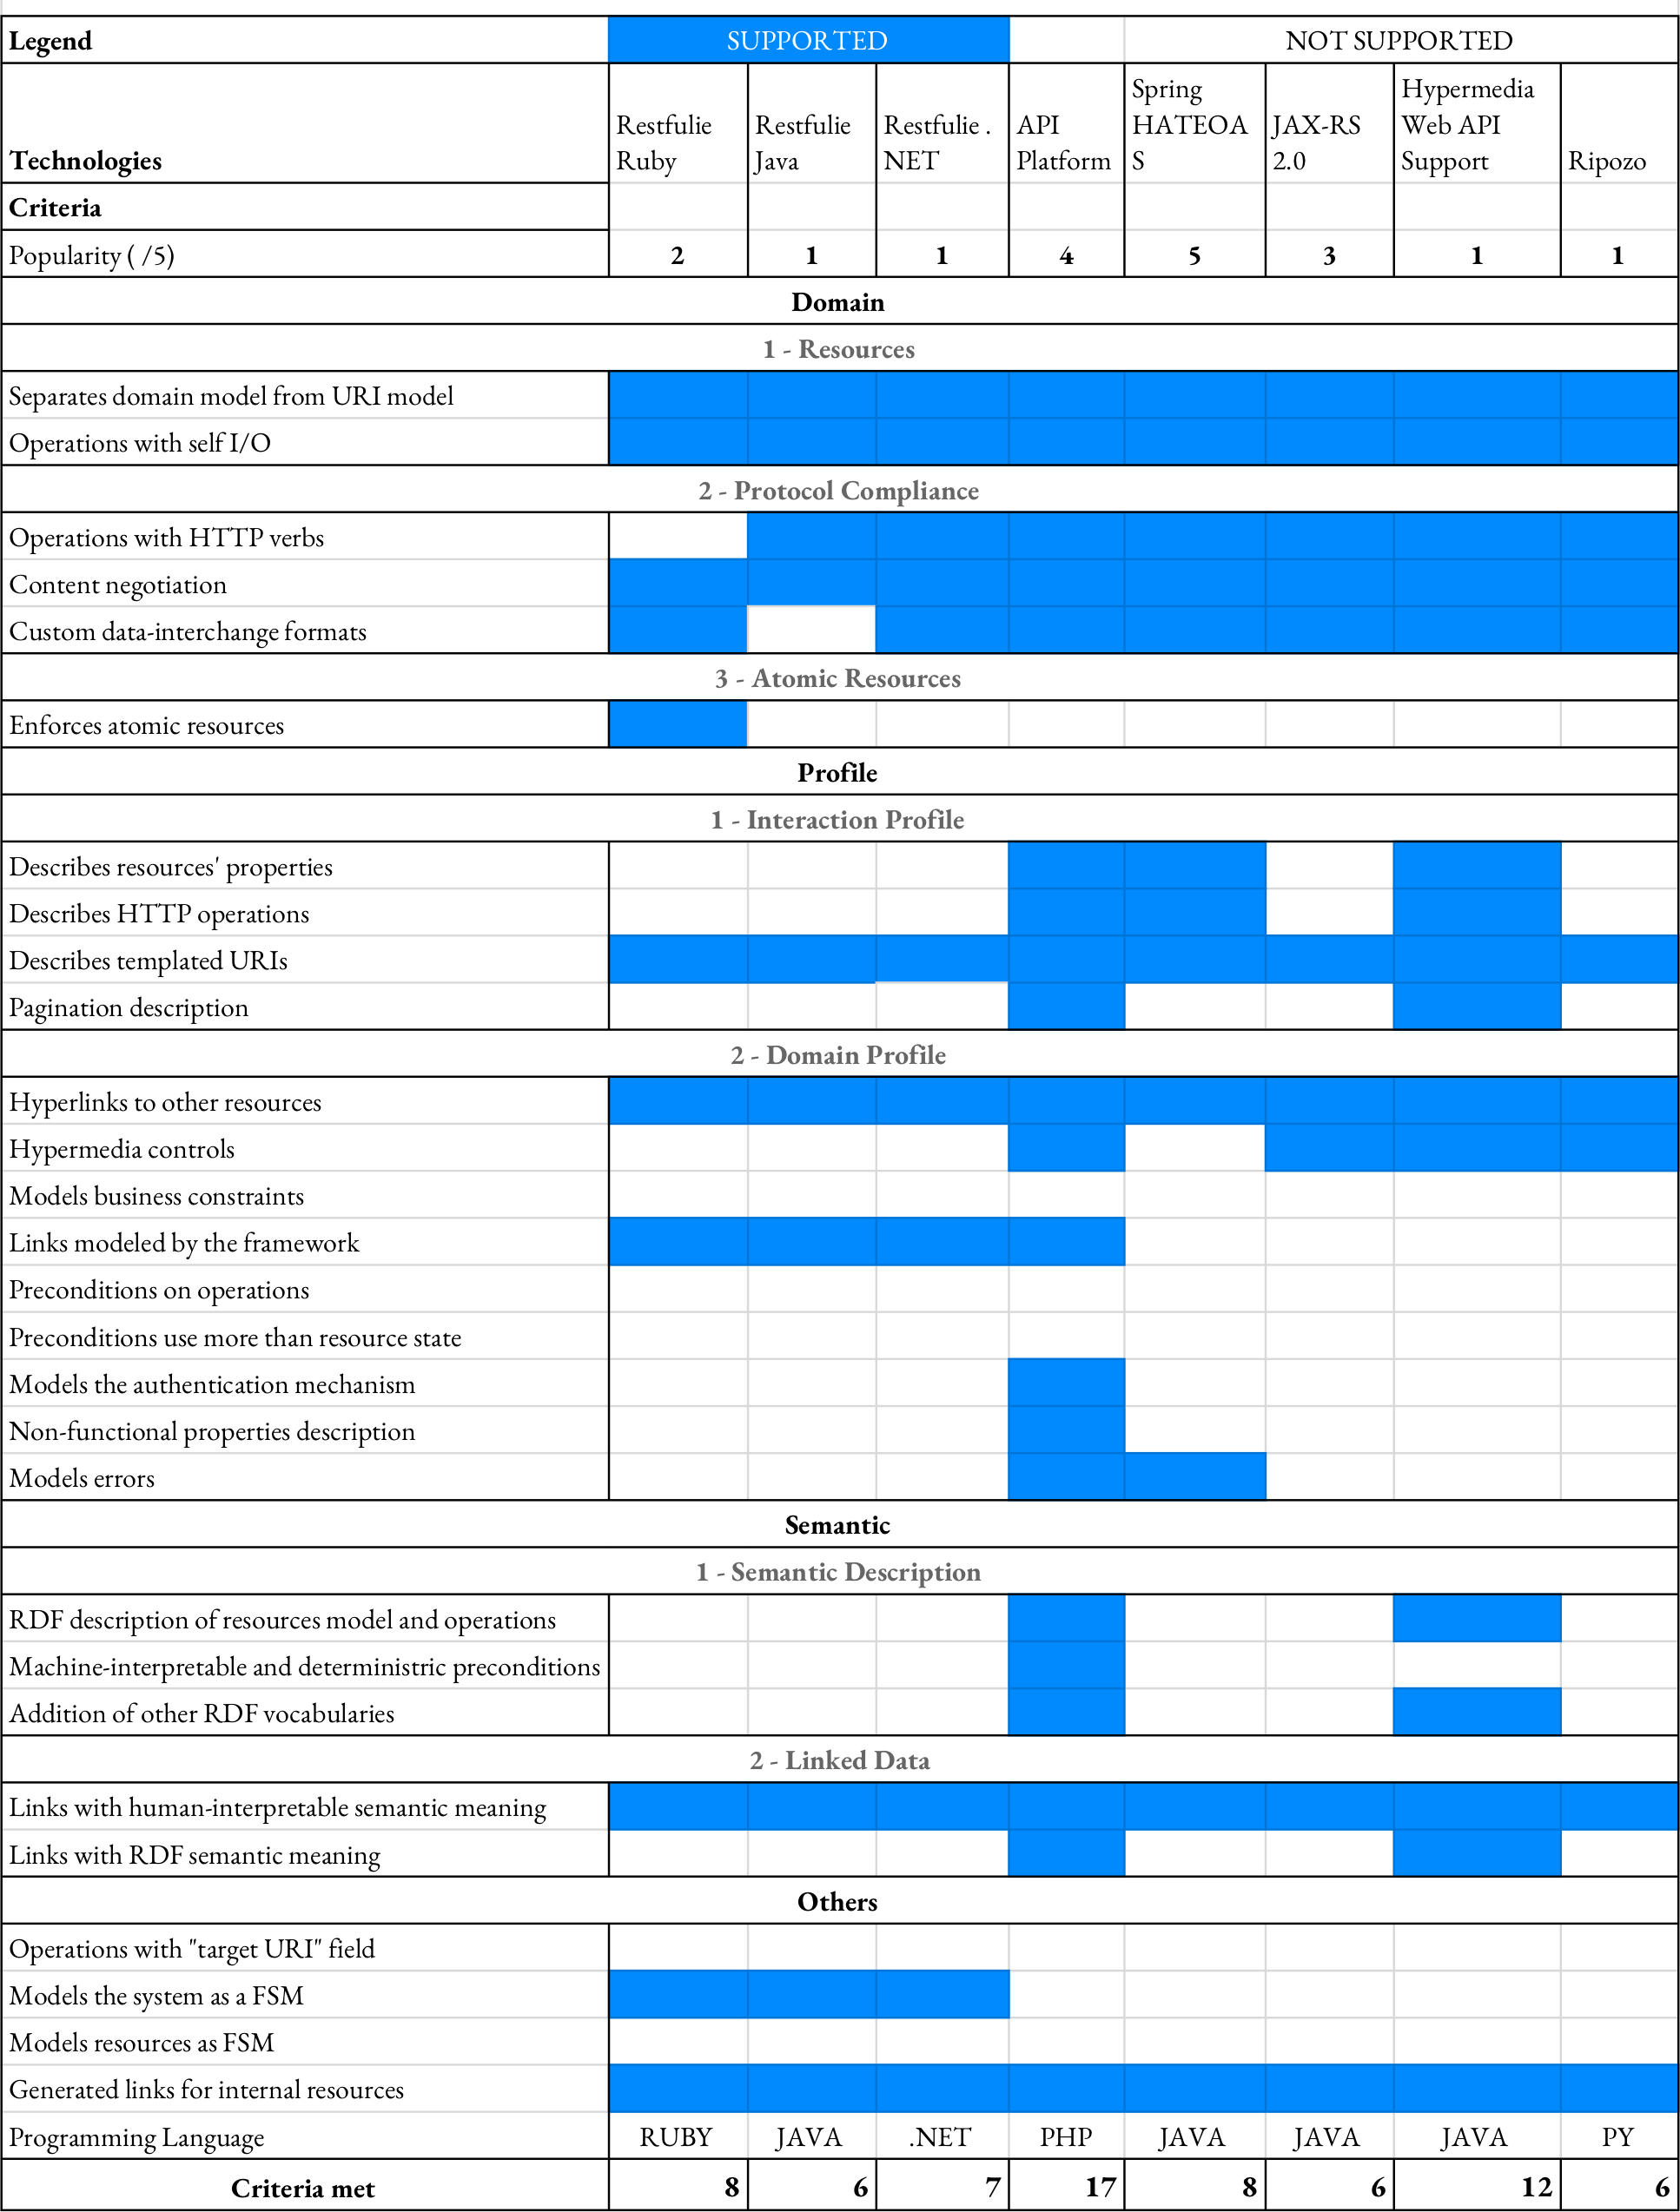
\includegraphics[width=1\textwidth]{figures/frameworks.png}
\label{frameworks-matrix}
\end{figure*}

\subsubsection*{Synthesis}
Despite the fact that only one framework enforces the \textit{Atomic Resources} constraint, all frameworks allow to reach the highest level of maturity on the \textit{design} dimension easily. This is because supporting the \textit{Atomic Resources} constraint only requires developers to use the data model of the resource as the input of write operations and as the output of read operations.\\
We notice that only \textit{API Platform} and \textit{Restfulie} offer a mechanism to model relations between resources from which links are automatically generated, instead of adding them programmatically in the response, thus increasing maintainability.\\
Otherwise, most frameworks do not ease the semantic and domain description of APIs. To us, this is the biggest challenge framework designers should tackle.\\
Last, as for IDLs, most creators of frameworks do not provide mechanisms to describe resources as state machines, thus not taking advantage of its benefits.

\section{Matrices usage example}

% To do well:
% [] figures should be concise and take as few space as possible -> to be optimized
% [X] example must be from a real example
% [X] justify the criteria that the technologies will have to meet -> to be validated by Johann & Olivier
% [X] if some technologies do not meet some criteria, explain why they can be chosen anyway
% [X] do not write a useless conclusion again (see section-4-archive.tex for an example)

In this section we present an insurance company's service that manage insurance contracts to demonstrate how the presented comparison matrices can be used in a real-world context. The domain of the project we present here is a lighten version of the combination of domains from projects we have done at XXX for former clients, who are big french insurance companies.

\subsection{Domain description}

To manage insurance contracts, the service holds five kinds of resources: (i) third-parties, (ii) contracts, (iii) warranties, (iv) cases and (v) services. Third-parties, who can for example be customers or contractors, enter into contracts with the insurance company. These contracts include warranties from the closed list of warranties that the company offers. Each warranty has options, let's take for example Person A who has the following warranties: (i) damage coverage with a deductible of \$500, and a maximum repair amount of \$30.000, (ii) premium vehicle loan in the event of immobilization of the damaged vehicle and (iii) reimbursement of the transport to the destination in the event of an accident, capped at \$2.000. A contract can have several cases. When an insured has a claim the company creates a case that holds the claim details and the services provided to the insured. For example, Person A has a car accident, he opens the insurance's web application and report a claim, which leads to the company opening a case. His car has been destroyed and he is expected to attend a family diner. So, on the app, he asks for a transport to his destination and a vehicle loan he will take delivery of at his destination the day after.

\subsection{Constraints on the technologies to select}

The service we describe have to communicate with both internal and external components. Internal components are front-end applications, such as mobile or web applications, and other kernel services, such as payments. External components are contractors APIs, for example taxi or mechanics companies. 

In the context of this service, there is a huge amount of business rules that determine (i) the warranties an insured can include in a contract and (ii) the available services for a case, based on the specificity of the given case and the warranties of the contract that the case is linked to. Writing and maintaining these rules both on the server and its clients would have been very costly. To keep business rules on the server-side only we decided to use the Hypermedia As The Engine Of Application State.

Because the project constitutes the core of the company's business, it should be future proof, which we believe includes being Linked Data compatible. Moreover, considering that the contractors that provide services are very diverse and numerous, the interactions with their APIs should leverage the possibilities offered by the use of RDF semantics, such as automatic discovery and composition. So, we looked for RDF-compatible technologies.

Because the project is core to the company, API clients will likely be built later on. So, the API should document its resources, resources' attributes, operations, URI templates, HTTP verbs, hypermedia controls and errors in a machine-interpretable way. Moreover, because the service applies the CQRS pattern\footnote{\url{https://martinfowler.com/bliki/CQRS.html}} we needed the IDL to allow associating each operation to its own input and output data model.

In the category of interchange format, the goal was to be as close as possible to what developers already know. So the format had to be based on JSON and entity-centric. The structure had to be as close as possible to an original JSON document.

Last, frameworks were considered based on the level of automation they provide.

\subsection{Selection of the technologies}

From these constraints we select a set of criteria and features to look for, listed in Table \ref{example-criteria}. We then count how many of these criteria each technology meet. Results are presented in Figure \ref{example-idl-results}, Figure \ref{example-dif-results} and Figure \ref{example-frameworks-results}. The three technologies matching the highest amount of selected criteria are highlighted in green for each kind of technology.

\begin{table*}[h]
\begin{minipage}[t]{0.5\linewidth}
\begin{tabular}{|c|}
 \hline
 \rowcolor{grey!10} \textbf{Design - 1. Resources} \\
 \hline
 Media types \\
 Models resources \\
 Operations with dedicated I/O \\
 Models resources' attributes \\
 \hline
 \rowcolor{grey!10} \textbf{Design - 2. Protocol Compliance} \\
 \hline
 Operations with HTTP verbs \\
 Custom data-interchange formats \\
 Content negotiation \\
 \hline
 \rowcolor{grey!10} \textbf{Profile - 1. Interaction Profile} \\
 \hline
 Describes resources' properties \\
 Describes HTTP operations \\
 Describes templated URIs \\
 Describes operations' HTTP verb \\
 \hline
 \rowcolor{grey!10} \textbf{Profile - 2. Domain Profile} \\
 \hline
 Hyperlinks to other resources \\
 Hypermedia controls \\
 Non-functional properties description \\
 Models errors \\
 \hline
 \rowcolor{grey!10} \textbf{Semantic - 1. Semantic Description} \\
 \hline
 RDF description of resources model and operations \\
 Addition of other RDF vocabularies \\
 \hline
 \rowcolor{grey!10} \textbf{Semantic - 2. Linked Data} \\
 \hline
 Links with human-interpretable semantic meaning \\
 Links with RDF semantic meaning \\
 \hline
 \rowcolor{grey!10} \textbf{Others} \\
 \hline
 JSON-based format \\
 Same structure as original JSON \\
 Entity-centric document \\
 \hline
\end{tabular}
\caption{Criteria to select the technologies in the example project}
\label{example-criteria}
\end{minipage}
\end{table*}

\begin{figure}[ht]
\caption{Results for interface description languages}
\centering
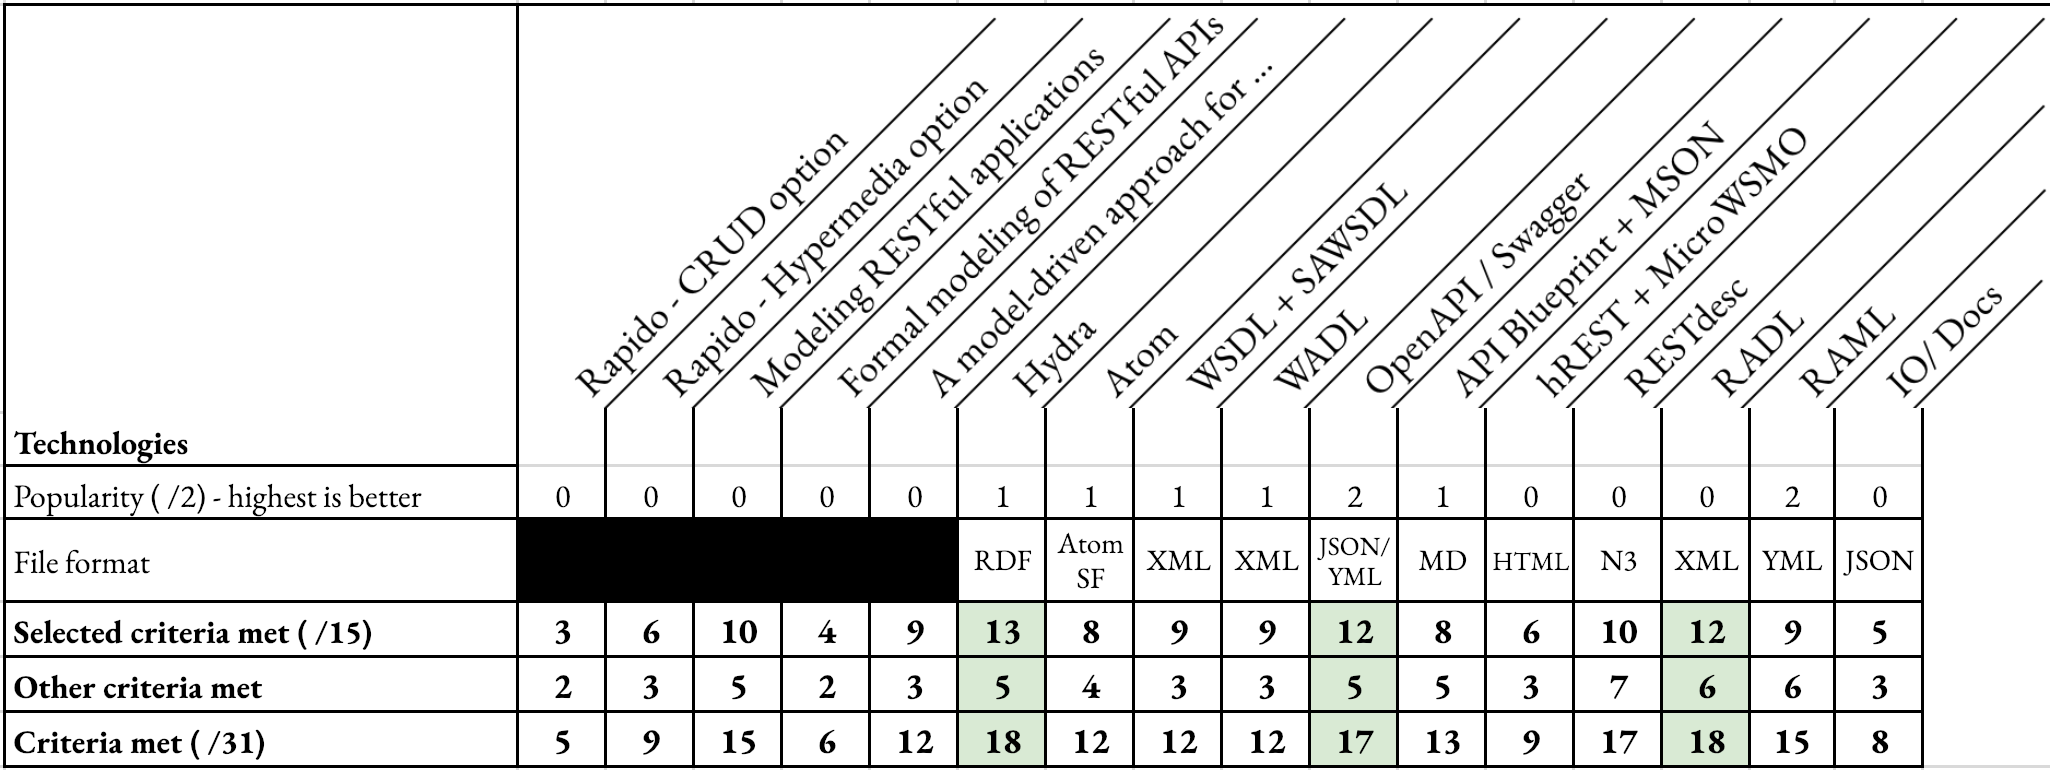
\includegraphics[width=1\textwidth]{figures/example-idl-results.png}
\label{example-idl-results}
\end{figure}

\begin{figure}[ht]
\caption{Results for data interchange formats}
\centering
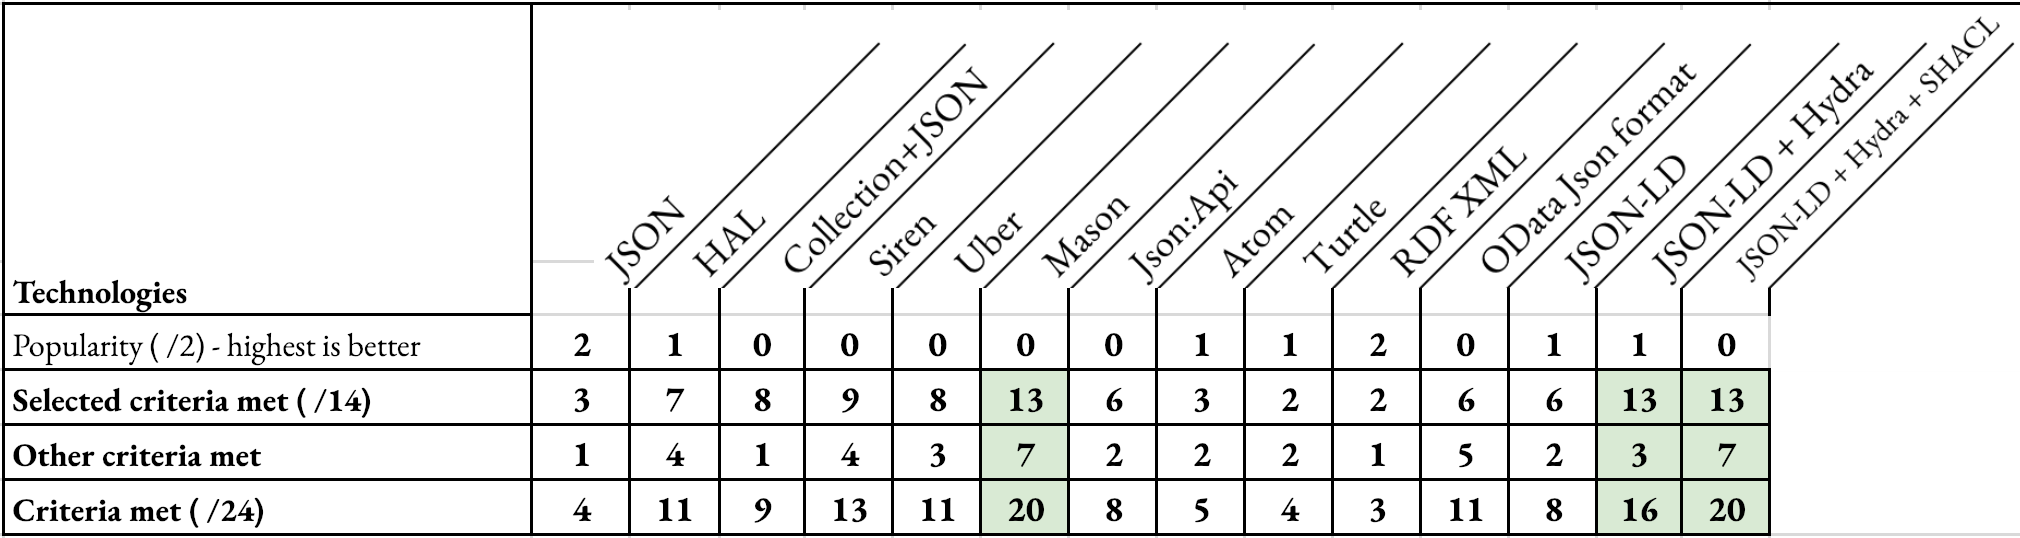
\includegraphics[width=1\textwidth]{figures/example-dif-results.png}
\label{example-dif-results}
\end{figure}

\begin{figure}[ht]
\caption{Results for implementation frameworks}
\centering
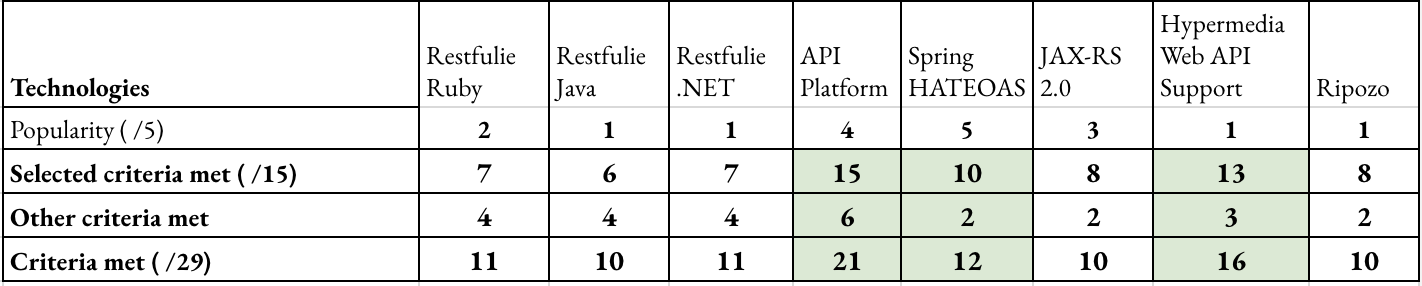
\includegraphics[width=1\textwidth]{figures/example-frameworks-results.png}
\label{example-frameworks-results}
\end{figure}

Technologies don't have to match every criteria to be selected. Most of the time, missing features can be implemented afterwards, or proposed to the maintainers of the technologies. A fine-grained analysis should be done on a per-feature basis.

\textbf{Interface Description Language.} Hydra, OpenAPI and RADL are the three technologies matching the highest number of selected criteria. However, no one matches every criteria. Hydra lacks the ability to describe non-functional properties and media-types, which can be done with other RDF vocabularies. RADL lacks the ability to semantically describe resources model and operations, errors and non-functional properties, which can also be done with other RDF vocabularies. On the other hand, OpenAPI does not support the description of hypermedia controls neither the usage of any RDF vocabulary, which is far more difficult to compensate. 

In the context of this project we chosen to use both Hydra and OpenAPI. OpenAPI because it has most features and is a must-have today because of its tooling and popularity. Hydra because it can be easily completed with other vocabularies and used with JSON-LD, when RADL is tight to XML.

\textbf{Interchange Formats.} Mason, JSON-LD + Hydra are the two technologies matching the highest number of selected criteria. JSON-LD + Hydra + SHACL can be ignored as it does not match more selected criteria than without SHACL. While JSON-LD + Hydra lacks the ability to describe non-functional properties, Mason does not allow to use RDF vocabularies. Again, being not compatible with RDF requires a lot more effort to compensate than finding another vocabulary. This explains why JSON-LD + Hydra was preferred over Mason in this context.

\textbf{Implementation frameworks.} API Platform, Spring HATEOAS and Hypermedia Web API Support \cite{salvadori2014framework} are the three technologies matching the highest number of criteria. Hypermedia Web API Support is immediately removed from the candidates because no public implementation is available. API Platform should be preferred over Spring HATEOAS because it matches five more criteria than Spring. However, developers of the companies we worked with know Java and not PHP. Moreover the Spring framework has a very good popularity with them which compensates the need to develop some features by hand. This is why we decided to go with Spring HATEOAS.

\subsubsection{Easing the selection of the technologies}

To ease the selection of the technologies with the comparison matrices, we developed an open-sourced web application\footnote{\url{https://antoinecheron.github.io/morice/}}. Users go through three steps: (i) selecting the kind of technologies they are looking for, (ii) selecting the criteria that are required and giving each criteria a value and then (iii) he is presented the results. Results is one table per kind of technology. In the table, the listed technologies are the ones that match the criteria that the user selected as required. Technologies are ranked by score. The score of one technology is the sum of the value of the criteria the technology meets.

This tool is intended to be improved in future works.
\section{Discussion} \label{sec:discussion}

% ANTOINE -> TODO

% TODO - from reviewer 2 : I agree with the fact that GraphQL is way more adopted than RDF-based semantic approaches, but how does it comes out from your previous analysis? GraphQL was not even mentioned before, and does not arise from the results. Please clarify how can one conclude that, by means of references and evidence from your analysis.

% TODO - from reviewer 2 : Finally, as a future work, authors could automatize the process to help developers in the form of a tool or wizard. -> already in progress

As indicated in the tables proposed in section \ref{sec:matrix} and in the example presented in the previous section, there is no framework yet available to build a semantic REST API. This section discusses, from our perspective, why there is no standard solution to meet all the criteria. These limits also make it possible to initiate research initiatives for the community. 

First, there is no IETF or W3C standard interchange format for building semantic REST APIs. In addition, none of the existing interchange formats support all the criteria described above, nor are they widely adopted, making it likely that new formats will emerge. For this reason, frameworks supporting semantic REST APIs will be forced to rely on formats that are prone to evolve, which will require additional effort and costs. This reduces the likelihood that developers will invest time in developing such features for their framework.

The second reason is that most developers ask for more support for GraphQL and streaming than for Semantic REST. We believe that this is due to two reasons. First of all, GraphQL and streaming are well understood and known, which is unfortunately less the case with RESTful semantic API concepts. Second, there is currently no tool that leverages the power of REST semantic APIs. Thus, being compatible with Semantic REST requires additional efforts to adapt client libraries and to train developers. We believe that with new tools, such as front-end clients, automated test libraries, improved documentation generation and HTTP clients such as Postman, developers would be more interested in semantic REST features.


\section{Related Work}

\vspace*{-0.2cm}

% OLIVIER -> TODO

% TODO : from reviewer 2 : By shortening Sec. 2 and 3 you make space for RELATED WORK, which is completely omitted. A quick search for "semantic rest apis survey" shows at least the following papers you must discuss:

% - Verborgh, Ruben, et al. "Survey of semantic description of REST APIs." REST: Advanced Research Topics and Practical Applications. Springer, New York, NY, 2014. 69-89.
% - Garriga, Martin, et al. "RESTful service composition at a glance: A survey." Journal of Network and Computer Applications 60 (2016): 32-53.

In \cite{verborgh_rest_2014}, and~\cite{7195633}, authors justify the need to provide a semantic description of REST APIs to avoid that programmers who develop client applications have to understand in depth several APIs from several providers. Based on this motivation, they survey academic approach to add semantic to such APIs description and technique to automatically compose restful services. %Compare to these works that  has been used to build the maturity model, we provide 

%Still todo
%APIComposer: Data-driven Composition of REST APIs


% Added by Antoine on December 31th -> TODO review
In \cite{serrano2017linked} authors present a framework for REST-service integration based on Linked Data models. First, API providers should semantically describe their REST services. Second, API consumers express data queries with SPARQL. Then, they use a middleware developed by the authors that can automatically compose API calls to respond to data queries with a RDF graph.
At the first step, authors needed to find and select an RDF-compatible Interface Description Language, which is precisely the kind of use-case our approach address. Because they could not find an existing one fitting their needs, they designed a new one by leveraging existing technologies such as MSM \cite{pedrinaci2010toward}, Hydra, RAML and OpenApi. %This new language cannot be classified in this paper as it is described on the surface and not documented.

In~\cite{Tuchinda:2011:BMD:1993053.1993058}, Tuchinda \textit{et al.} describe a programming-by-demonstration approach to build mashups by example. Instead of requiring a user to select and customize a set of widgets, the user simply demonstrates the integration task by example. Their approach addresses the problems of extracting data from web sources, cleaning and modeling the extracted data, and integrating the data across sources. It illustrates the benefits of getting meta-data on top of services to improve the definition of mashups and decrease the coupling between information system building blocks and the complexity of  developing mature Semantic REST APIs. In~\cite{10.1007/978-3-642-17694-4_11}, Duke \textit{et al.} propose an approach to reduce the complexity for describing, finding, composing and invoking semantic rest services. They mainly provide an approach where they show how they can combine services when they get semantic information. 

Other research efforts were done to lower the entry barrier for developing mature Semantic REST APIs. Among them is the semi-automatic annotation of web services as done by Patil \textit{et al}. in \cite{patil2004meteor}. Their contribution could help significantly increase the number of semantically described services, in case their work is open-sourced and updated to support nowadays popular technologies.

GraphQL and API streaming technologies are very popular. 
%GraphQL is now a specific topic of the API Days conference while REST semantic or Linked Data applications are not. 
These technologies are seen as concurrent to REST APIs for a part of the community. 
We argue that when building large scale application semantic REST APIs offers greater flexibility and performance.

% Works going in the same direction :
% Tools to help semantically annotate documents
% Karma tool : https://dl.acm.org/citation.cfm?id=1993058
% http://sweet.kmi.open.ac.uk/
\section{Conclusion}

\vspace*{-0.2cm}

In this paper, we have presented three comparison matrices that assist architects in choosing Semantic REST APIs enabling technologies that meet their needs.
Through a real example, we have illustrated how the use of these matrices simplifies the choice of these technologies. 
As stated in the paper, technologies should be chosen not only according to the number of criteria they meet, but also according to the specific needs of the project. 
To facilitate this selection, we have developed an assistant available online.

We also pointed out some interesting features missing in current technologies.
The description of constraints and conditions indicating the availability of state transitions is ignored by IDLs, vocabularies, interchange formats and frameworks. On the other hand, resource modeling as FSM is not available in most frameworks.
More importantly, well-known tools do not take advantage of the power of Semantic REST APIs to provide additional and useful features.

Based on these findings, we identify areas for improvement in the tools around Semantic REST APIs that we believe can increase its adoption. By leveraging the semantic description and advertising of state transitions and non-functional properties, automated testing tools can become smarter, REST client libraries can lower the coupling with the server and automate tasks such as login, and middleware can automatically create responses from the composition of several APIs.
%
% ---- Bibliography ----
%
% BibTeX users should specify bibliography style 'splncs04'.
% References will then be sorted and formatted in the correct style.
%
% \bibliographystyle{splncs04}
% \bibliography{mybibliography}
%

\bibliographystyle{splncs04}
\bibliography{bibliography}

\end{document}
